% Finished September 11, 2013
% Put into VUW Thesis format Wednesday 2 April 2014

\documentclass[12pt, a4paper, twoside, openright]{book}

\usepackage{vuwthesis} % sets up some local things, mostly the front page

\setlength{\intextsep}{12pt} % set space above and below in-line float
\setlength{\abovecaptionskip}{0pt} % set space between figure and caption.

\usepackage{url}

\usepackage{amssymb, amsmath}
%\usepackage{mathtools}
\usepackage{tikz}
\usetikzlibrary{calc}

\newcommand{\beff}{\ensuremath{b_{\mathrm{eff}}}}
\newcommand{\bmin}{\ensuremath{b_{\mathrm{min}}}}
\newcommand{\bmax}{\ensuremath{b_{\mathrm{max}}}}
\newcommand{\bfar}{\ensuremath{b_{\mathrm{far}}}}
\newcommand{\beffh}{\ensuremath{b_{\mathrm{eff}}} = \left< \frac{1}{b} \right>^{-1} }
\newcommand{\beffhf}{\ensuremath{b_{\mathrm{eff (flat)}}} = \left< \frac{1}{b} \right>^{-1} }
\newcommand{\beffha}{\ensuremath{b_{\mathrm{eff}}} = \left< \sqrt{1 + |\nabla h|^2} / {b} \right>^{-1} }
\newcommand{\beffm}{\ensuremath{b_{\mathrm{eff}}} = \left< b \right> }



%\usepackage{marvosym}

\usepackage{etoolbox}
\newtoggle{compilealone}
\toggletrue{compilealone}

\title{Chapter 8: Numerical Testing}
\author{Nat Lund}

\begin{document}
\chapter{Numerical Testing}\label{C:numerics}

We have derived two analytic formulae for the effective slip length of a mixed slip surface, using two different mathematical techniques.
The homogenized effective slip length is exact in the limit of vanishing period, and is expected to be a useful approximation if a physical system is `near the limit'.
A way to quantify `nearness to the limit' is to
compare the magnitudes of the relevant length scales of the system: the period $L$ of the surface patterning, and the domain height $P$.  Thus, a physical system is near the limit if:
\begin{equation}
L \ll P
\end{equation}
Our perturbative effective slip lengths were also derived with the assumption that $L \ll P$; furthermore, the $\beffm$ expression is expected to be a good approximation when $b \ll  L$.

We wish to test our predictions against the `true' slip lengths of physical systems as they get closer and closer to the relevant limits.
Ideally, one would measure effective slip lengths in physical experiments.  
Such experiments are beyond the scope of this thesis.  However, the next best thing are numerical simulations carried out by a computer.  Therefore, in this chapter we compare our predicted $\beff$ expressions with effective slip lengths derived from numerical simulations.



%We cannot precisely quantify `nearness to the limit': In our model we have two length scales, the period of slip variation $L$, and the minimum slip length $\bmin$, and our formula is exact in the limit $L \to 0$.  All we can say is that a system is `near the limit' if $L$ is `near to 0' \emph{compared to $\bmin$.} That is, a system is near the limit if $L \ll \bmin$.

%Our formula predicts an effective slip length; we wish to test our prediction against the `true' slip length. In particular, we wish to compare our prediction with the true slip lengths of systems as they move ever further from the limit.  The only true effective slip length is one measured in a physical experiment.  Such experiments are beyond the scope of this thesis.  However, the next best thing is a computer experiment, usually referred to as a numerical simulation.

\section{Finite Element Modelling}

Perhaps the most powerful and versatile numerical method for solving partial differential equations is Finite Element Modelling (FEM).  Many industrial-strength implementations are available; we chose the free and open-source package \textbf{FreeFem++}, available from \url{www.freefem.org} \cite{freefem++}.

The input to FEM software is a precise description of the model, including the size and shape of the domain, and the equations that hold on the domain and its boundaries. The output of an FEM simulation is a velocity field on the domain.  

In our FEM simulations, we used a model with Laplace's equation holding on a rectangular domain of height $P$, with a fixed shear rate $\dot{\gamma} $ at the top of the domain, periodic boundary conditions on the sides of the domain, and the full tensor slip boundary condition at the bottom of the domain.  See Figure (\ref{FEMdomain}).

\begin{figure}[ht]
\centering
\begin{tikzpicture}

\draw [domain=0:4.5,samples=200] plot (\x,{ 0.2 * sin(7*\x r)} );
\draw[dashed] (0,0) -- ++(0,2) (4.5,0) -- ++(0,2);
\draw[dotted] (0,2) -- ++(4.5,0);

\node at (2.25,-0.5) {$\Gamma_b $};
\node at (5,1) {$\Gamma_0 $};
\node at (-0.5,1) {$\Gamma_0 $};
\node at (1.25,2.5) {$\Gamma_{\mathrm{top}} $};
\node at (2.25,1) {$\Omega $};

\draw[very thick,->] (3,2) -- ++(0,0.5);
\draw[very thick,->] (3,2.5) -- ++(0.5,0);
\draw [dotted](3,2) -- ++(0.6,0.6);
\node at (3.5, 2.3)[right]{shear rate = $\dot{\gamma}$};

\end{tikzpicture}
\caption{Domain $\Omega$ with rough slip boundary $ \Gamma_b $, top boundary $\Gamma_{\mathrm{top}}$ and periodic side boundaries $\Gamma_0$.}\label{FEMdomain}
\end{figure}

For convenience when working with slip boundary conditions, in this thesis we adopted the convention that the unit normal vector $\vec{n}$ on the surface points `up' into the fluid, that is, \emph{into} the domain. (An increase in $x$ velocity with increasing $z$ gives a positive velocity gradient $\partial u /\partial z$.  On a flat surface, the convention of the inward-pointing $\vec{n}$ ensures that the velocity gradient in the direction of $\vec{n}$, $\partial u/\partial n$, has the same sign (and magnitude) as $\partial u/ \partial n$.)  A consequence is that the normal vector $\vec{n}$ on the top boundary points \emph{down.}

The flow is shear-driven only.  The top fixed-shear boundary condition can be expressed in terms of the deformation rate tensor:
\begin{equation}
 2 \mathbf{E}(\vec{u}) \cdot \vec{n} = (- \dot{\gamma}, 0)
\end{equation}
(The negative sign is due to the downward-pointing $\vec{n}$ on the top boundary.)

Then the derivation of Section 6.2.3 (page 126) can be augmented with the top shear boundary condition to get:
\begin{equation}
\int_{\Gamma_b} \frac{1}{b} \vec{u} \cdot \vec{g} +
\int_{\Gamma_{\mathrm{top}}} (-\dot{\gamma},0) \cdot \vec{g} = 
2 \int_{\Omega} \mathbf{E}(\vec{u}) : \mathbf{E}(\vec{g}) +
\frac{1}{\mu} \int_{\Omega}  \nabla p \cdot \vec{g}
\end{equation}
However, the flow is shear-driven only, with no pressure drop across the domain, so the integral containing the pressure gradient vanishes, leaving:
\begin{equation}
\int_{\Gamma_b} \frac{1}{b} \vec{u} \cdot \vec{g} -
\int_{\Gamma_{\mathrm{top}}} (\dot{\gamma},0) \cdot \vec{g} = 
2 \int_{\Omega} \mathbf{E}(\vec{u}) : \mathbf{E}(\vec{g})
\label{eq:FEMformula_inward}
\end{equation}
Note that the viscosity has vanished due to the periodicity of the pressure.

While our convention of an inward-pointing normal vector $\vec{n}$ was appropriate for studying slip, an \emph{outward-pointing} unit normal is the more common convention in mathematics, including in finite element modelling.  To use the formula of Equation (\ref{eq:FEMformula_inward}) in Freefem++, we must change to the outward-pointing convention. This alters the boundary conditions by a negative sign to $ 2 \mathbf{E}(\vec{u}) \cdot \vec{n} = -\frac{1}{b} \vec{u} $ and $2 \mathbf{E}(\vec{u}) \cdot \vec{n} = (\dot{\gamma}, 0) $, which amounts to multiplying $b$ and $\dot{\gamma}$ by $-1$ in Equation (\ref{eq:FEMformula_inward}).  Thus, the variational formula used for the Freefem++ simulations was:
\begin{equation}
2 \int_{\Omega} \mathbf{E}(\vec{u}) : \mathbf{E}(\vec{g}) -
\int_{\Gamma_{\mathrm{top}}} (\dot{\gamma},0) \cdot \vec{g} +
\int_{\Gamma_b} \frac{1}{b} \vec{u} \cdot \vec{g} = 0
\end{equation}
The shear rate $\dot{\gamma}$ was set to one.



\begin{figure}[ht]
\begin{center}
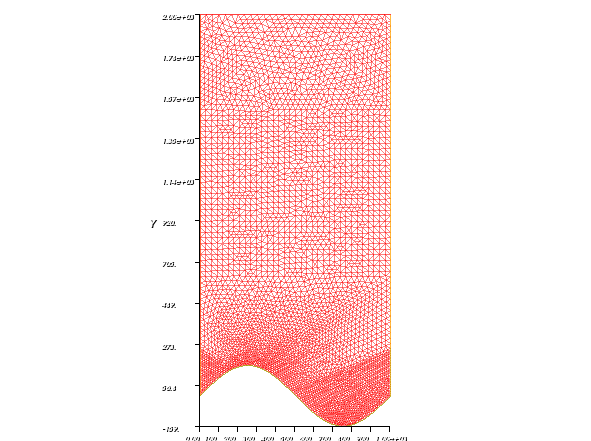
\includegraphics[scale=0.5, trim=4cm 0cm 4cm 0cm, clip=true]{FEM_mesh_1.png}
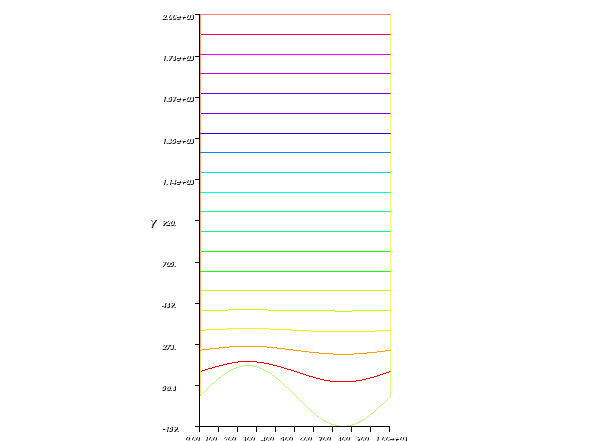
\includegraphics[scale=0.5, trim=4cm 0cm 4cm 0cm, clip=true]{FEM_streamlines_1.png}
\end{center}
\vspace{1em}
\begin{center}
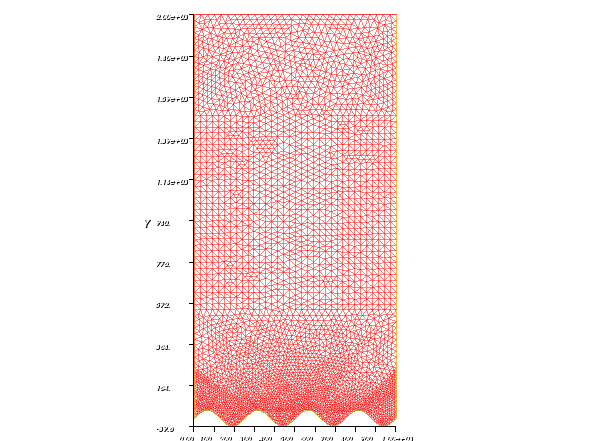
\includegraphics[scale=0.5, trim=4cm 0cm 4cm 0cm, clip=true]{FEM_mesh_4.png}
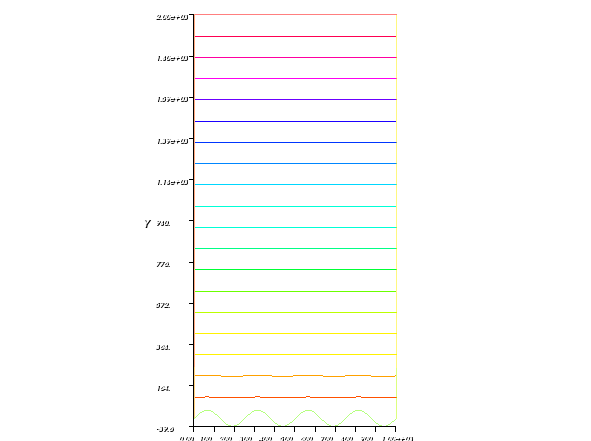
\includegraphics[scale=0.5, trim=4cm 0cm 4cm 0cm, clip=true]{FEM_streamlines_4.png}
\end{center}

\caption{The mesh (left) and velocity streamline plot (right) for FEM simulations on a domain with a rough slip surface with one period (top) and four periods (bottom).}
\label{FEMmesh4}
\end{figure}

\clearpage

Several simulations were done, with different period lengths, on both sinusoidal and flat slip boundaries.  An FEM simulation has a mesh defined on the domain, specifying the points at which a velocity solution is found.  An adaptive mesh was used, so that each full sine cycle always had at least six mesh points on it, even for very short period lengths.

The mesh and corresponding velocity streamline plot for a couple of simulations are shown in Figure (\ref{FEMmesh4}).  Notably, within a period length or two of the sinusoidal surface, the velocity has become uniform horizontal flow.
%but quickly settle down to uniform flow in the $x$ direction only:  Within about a single period length of the surface, the streamlines are almost perfectly flat.

\vspace{1em}
The top of the domain, at height $P$ above the slip surface, is known as the far field.  The velocity and shear rate in the far field, together with the height, define an effective slip length, as described in Chapter 1.  We shall denote this FEM far-field effective slip length as $\bfar$.  In \textbf{all of our simulations}, the far-field velocity turned out to be constant and in the $x$ direction only, even when the period was as large $\frac{1}{2}$ of the domain height.  Therefore, $\bfar$ was always a well-defined single value.



\subsection{Flat Surface}

We start with the simplest case of a flat surface, with a binary slip patterning consisting of alternating stripes of high slip ($\bmax$) and low slip ($\bmin$) material.  The stripes are of equal width; two stripe widths equal the period $L$.

\clearpage
\subsubsection{Harmonic Mean Formula}
The homogenization analysis yielded $\beffha$, which is expected to be a good approximation in the limit $L \ll P,b$.  The perturbation analysis yielded $\beffh$ --  the same formula simplified for flat surfaces.  Therefore, we set $\bmax = P$ and $\bmin = \frac{1}{5}P$, and ran a series of FEM simulations for different values of $L$, starting with $L = \frac{1}{2}P$, going down to $L = \frac{1}{320}P$.  The far-field FEM effective slip length $\bfar$ was calculated for each simulation.  The results are plotted in Figure (\ref{FEMplotflatL}).

%\clearpage
\begin{figure}[ht]
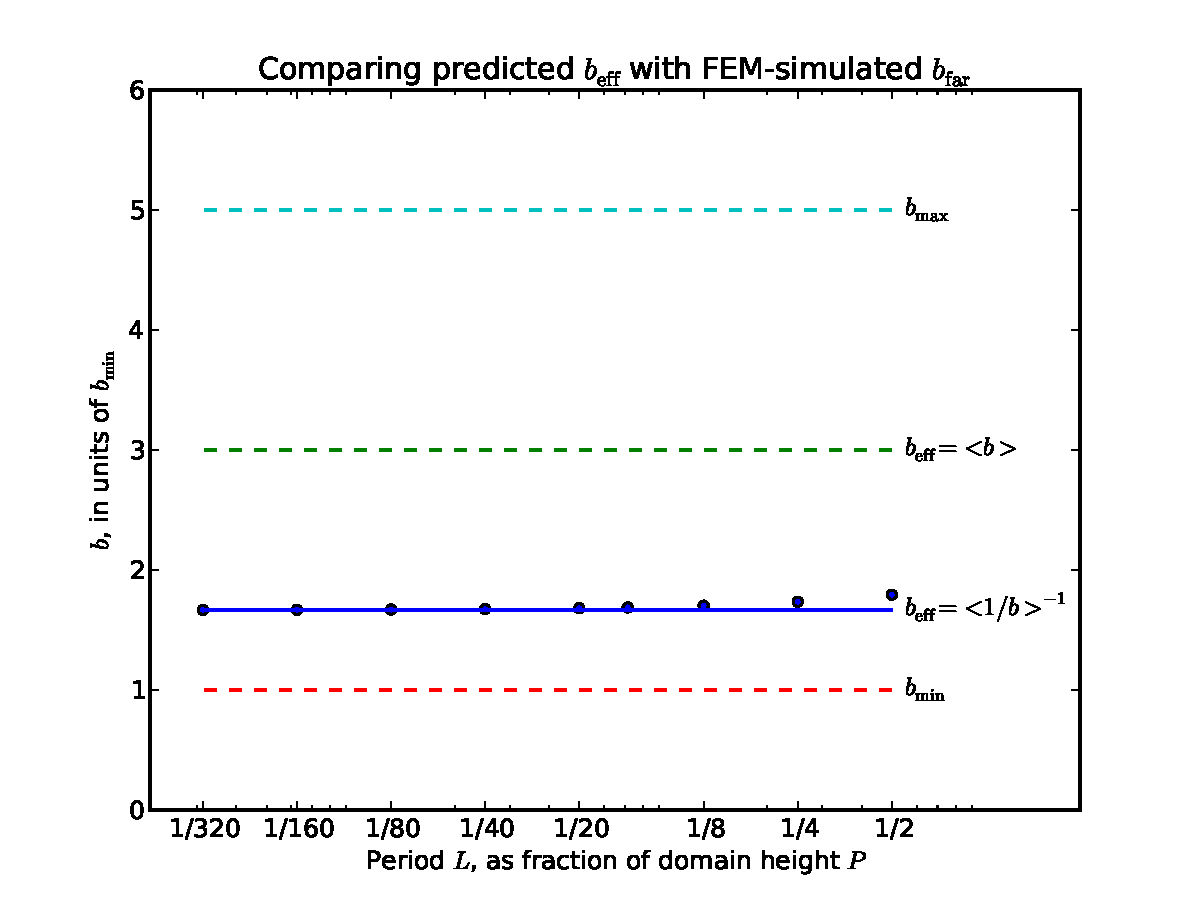
\includegraphics[scale=0.595]{Lund_Thesis_FEM_plot_flat_L}
% Absurd scale factor is to suppress the error message!
\caption{Comparison of numerical $\bfar$ values with predicted $\beff$ for different period sizes, with $b \sim P$.  The dots are values of $\bfar$.  The solid line is the $\beffh$ prediction.}\label{FEMplotflatL}
\end{figure}

As Figure (\ref{FEMplotflatL}) shows, if $b \sim P$, the harmonic mean $\beffh$ formula is an excellent approximation of $\bfar$ if $L \ll P$, and still a good approximation even if $L \sim P$.  Thus, at least in this numerical simulation, the requirement $L \ll P$ is in practice met by the condition $L \leq \frac{1}{10}P$.

\clearpage
\subsubsection{Simple Mean Formula}

The perturbation analysis also yielded a formula $\beffm$ in the limit of vanishing slip length.  This simple area-weighted mean was derived assuming $L \ll P$, and is expected to be a good approximation to $\bfar$ in the limit $b \ll L \ll P$.  To explore this, we ran a series of FEM simulations with fixed $L = \frac{1}{10}P$, and $\bmax$ varying from $\bmax = P$ down to $\bmax = \frac{1}{400}P$.  The $\bfar$ of each simulation is plotted as a dot in Figure (\ref{FEMplotflatb}).
%\clearpage

\begin{figure}[ht]
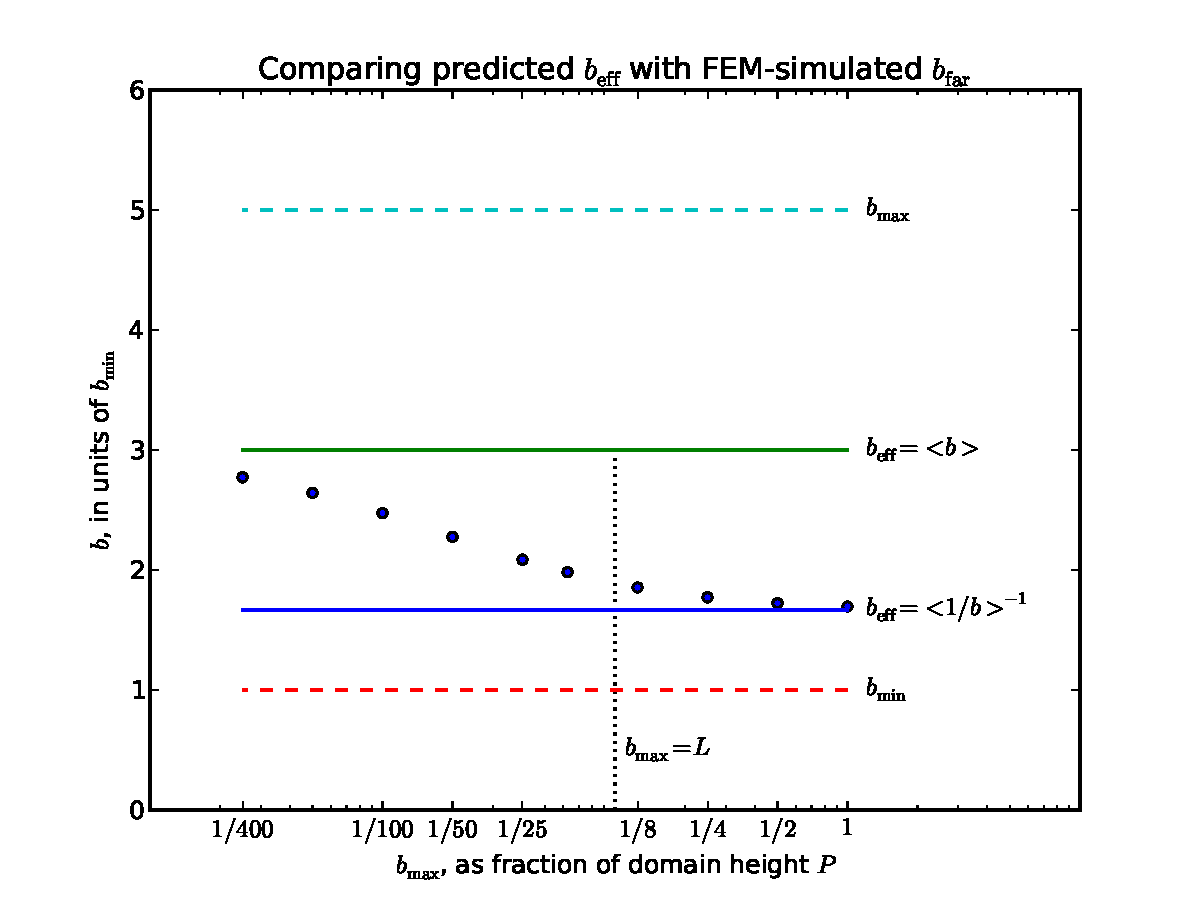
\includegraphics[scale=0.595]{Lund_Thesis_FEM_plot_flat_b}
% Absurd scale factor is to suppress the error message!
\caption{Comparison of numerical $\bfar$ values with $\beff$ predictions, for different values of $\bmax$, with $L = \frac{1}{10}P$. The dots are values of $\bfar$. The lower solid line is the $\beffh$ prediction, and the upper solid line is $\beffm$ prediction.  The vertical dotted line indicates where $\bmax = L$.}\label{FEMplotflatb}
\end{figure}

The values of $\bfar$ in Figure (\ref{FEMplotflatb}) demonstrate a gradual transition from the regime where $\beffh$ applies to the regime where $\beffm$ applies.
Figure (\ref{FEMplotflatb}) affirms that $\beffh$ is an excellent approximation in the regime $L \ll b,P$, and reveals that $\beffh$ is a surprisingly good approximation in the regime $ L \sim b \ll P$.
 The `limit of vanishing slip length' is shown to be quite a strong condition: The regime $b \approx \frac{1}{1	0} L \ll P$ is a `transition regime', with the $\bfar$ values midway between the simple mean and the harmonic mean; the simple mean is not a good approximation until $\bmax \leq \frac{1}{40}L$.

\clearpage
\subsection{Rough Surface}

The FEM testing on a flat surface showed our harmonic mean $\beffh$ formula to be an excellent approximation in the regime $L \ll P, \bmax$.  We now wish to investigate the importance of the arc-length correction -- the correction due to the increased area of liquid-solid contact on a rough surface.

To that end, we ran a series of FEM simulations with sinusoidal surfaces. Each surface was a corrugation with the standard sine-wave profile -- the amplitude and period are always in the ratio $1:2\pi$.  The slip length varied in a binary fashion, with high slip in the valleys of the sinusoid, and low slip on the peaks of the sinusoid.  This models a nanograting with air pockets in the grooves.  The flow was shear-driven by a fixed shear rate, and the slip lengths were fixed at $\bmin = \frac{1}{5} P, \; \bmax = P$.  A schematic appears in Figure (\ref{FEMroughmodel}).

\begin{figure}[ht]
\centering
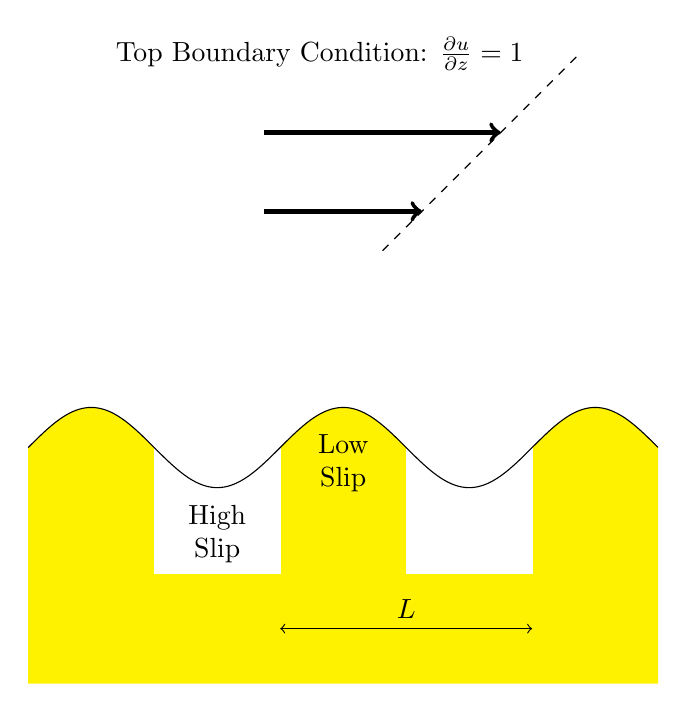
\begin{tikzpicture}
\node at (3.7,5) {Top Boundary Condition: $\frac{\partial u}{\partial z} = 1 $};

\draw[->, ultra thick] (3,4) -- ++(3,0);
\draw[->, ultra thick] (3,3) -- ++(2,0);
\draw[dashed] (3,2.5) ++(1.5,0) -- ++(2.5,2.5);

% \L = 3.2; length of period
\fill [color=yellow,domain=0:8,samples=200] plot (\x,{ (3.2 /6.2823) * sin( 6.2832 *\x / 3.2 r)} ) -- ++(0,-3) -| (0,0);

\draw[color=white,fill=white] (1.6,0) rectangle ++(1.6,-1.6);
\draw[color=white,fill=white] (4.8,0) rectangle ++(1.6,-1.6);

\draw [domain=0:8,samples=200] plot (\x,{ (3.2 /6.2823) * sin( 6.2832 *\x / 3.2 r)} );

\draw[<->] (3.2,-2.3) -- node[above] {$L$} ++(3.2,0);

\renewcommand{\baselinestretch}{1.00}
\node at (2.4,-1.1) [align=center] {High \\ Slip};
\node at (4,-0.2) [align=center] {Low\\ Slip};


\end{tikzpicture}
\caption{Schematic of the FEM model with corrugated mixed-slip surface.}\label{FEMroughmodel}
\end{figure}

A series of FEM simulations were done with different periods of the sinusoidal corrugation, starting from $L = \frac{1}{2}P$, down to $L = \frac{1}{200}P$. The $\bfar$ from each simulation appears as a dot in the plot of Figure (\ref{FEMplotsine}).

\begin{figure}[ht]
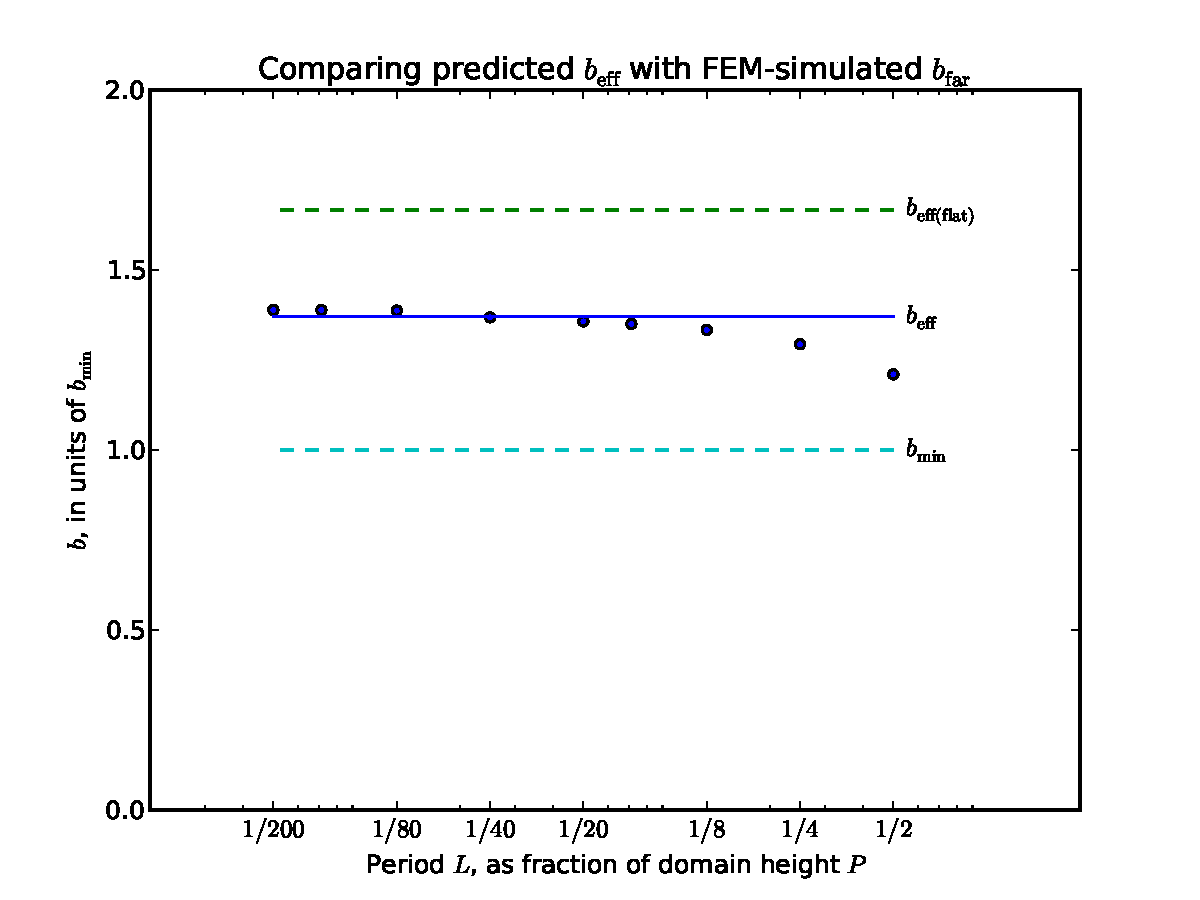
\includegraphics[scale=0.595]{Lund_Thesis_FEM_plot_sine}
% Absurd scale factor is to suppress the error message!
\caption{Comparison of numerical $\bfar$ values with $\beff$ predictions for \textbf{sinusoidal} surfaces for different periods, with $b\sim P$. The dots are values of $\bfar$. The solid line is the  $\beffha$ prediction.  The upper dashed line is the $\beffhf$ predicted if the surface were assumed to be flat.}\label{FEMplotsine}
\end{figure}

Figure (\ref{FEMplotsine}) clearly shows the significance of the arc length correction: The full $\beffha$ expression with arc length correction is shown as the solid line, and the $\bfar$ values converge on this line as $L$ gets smaller. The $\beffhf$ calculated if the surface were assumed to be flat is shown as the upper dotted line.  Thus, if $b\sim P$, then the full $\beff$ prediction is an excellent approximation when $L \ll P$.

To better test the accuracy of the $\beff$ prediction, we calculated the differences between the $\bfar$ values and $\beff$, expressed as a percentage of $\beff$.  The resulting percentage differences are plotted in Figure (\ref{FEMplotsinepcnt}). 

\clearpage
\begin{figure}[ht]
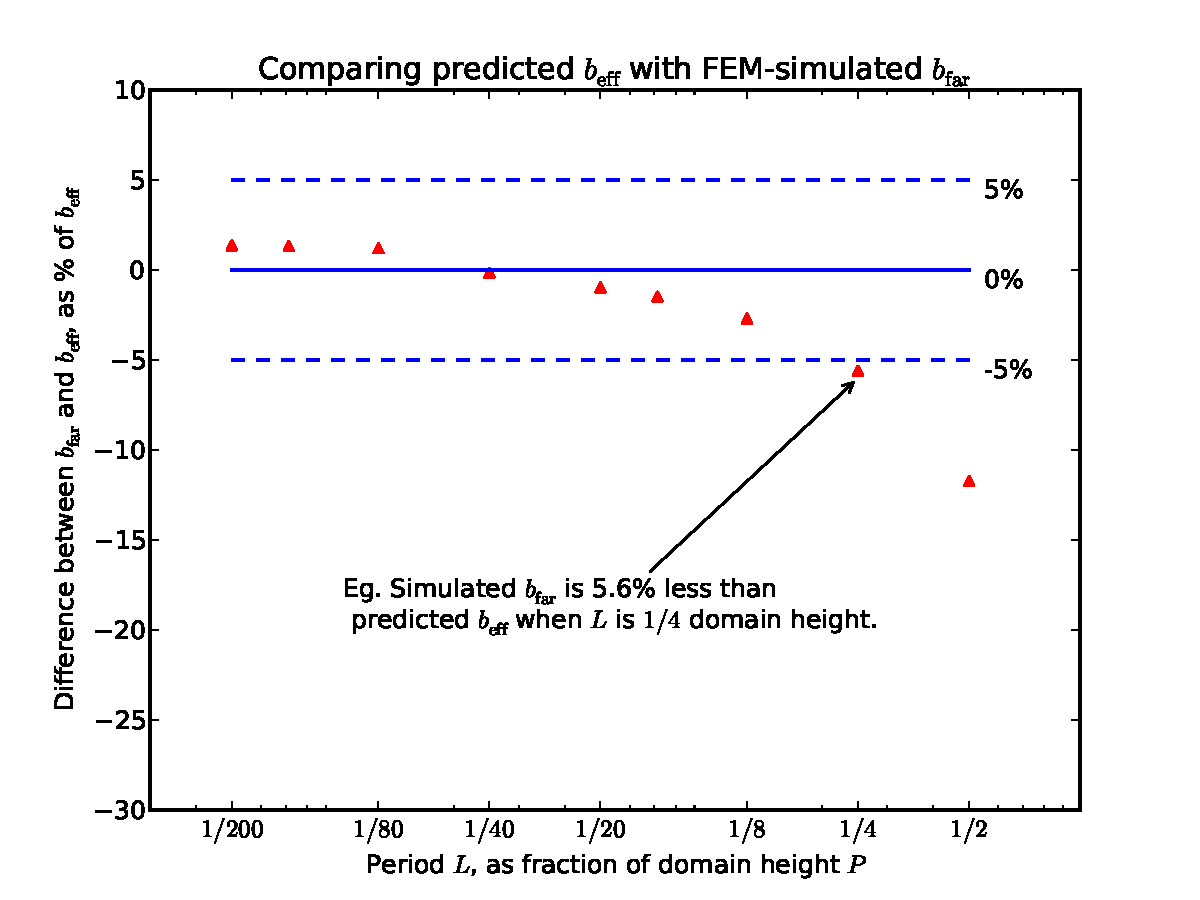
\includegraphics[scale=0.595]{Lund_Thesis_FEM_plot_sine_pcnt}
% Absurd scale factor is to suppress the error message!
\caption{Percentage comparisons between numerical $\bfar$ values and contact-area-corrected $\beffha$ predictions. The dots are values of $\bfar$, expressed as the percentage $(\bfar -\beff)/\beff \times 100 $. }\label{FEMplotsinepcnt}
\end{figure}

The percentage differences of Figure (\ref{FEMplotsinepcnt}) reveal that our contact-area-corrected $\beffha$ prediction for rough surfaces is accurate to within a few \% when $L \ll P, \bmax$.
For example: Accurate to within 5\% when $L \leq \frac{1}{5}P$, and within 1\% when $L$ is less than 5\% of $P$.

The slip lengths in these FEM simulations were calculated with respect to the $z=0$ line, about which the sinusoids oscillate.  In Chapter 3 we noted the ambiguity in the definition of slip length -- does the surface begin at the $z=0$ line or at the tops of the sine wave peaks?  To investigate this issue, we recalculated the measured slip lengths with respect to the \textbf{tops of the peaks}.  These are plotted as the crosses in Figure (\ref{FEMplotsinecorr}) (along with the `uncorrected' slip lengths).

\clearpage
\begin{figure}[ht]
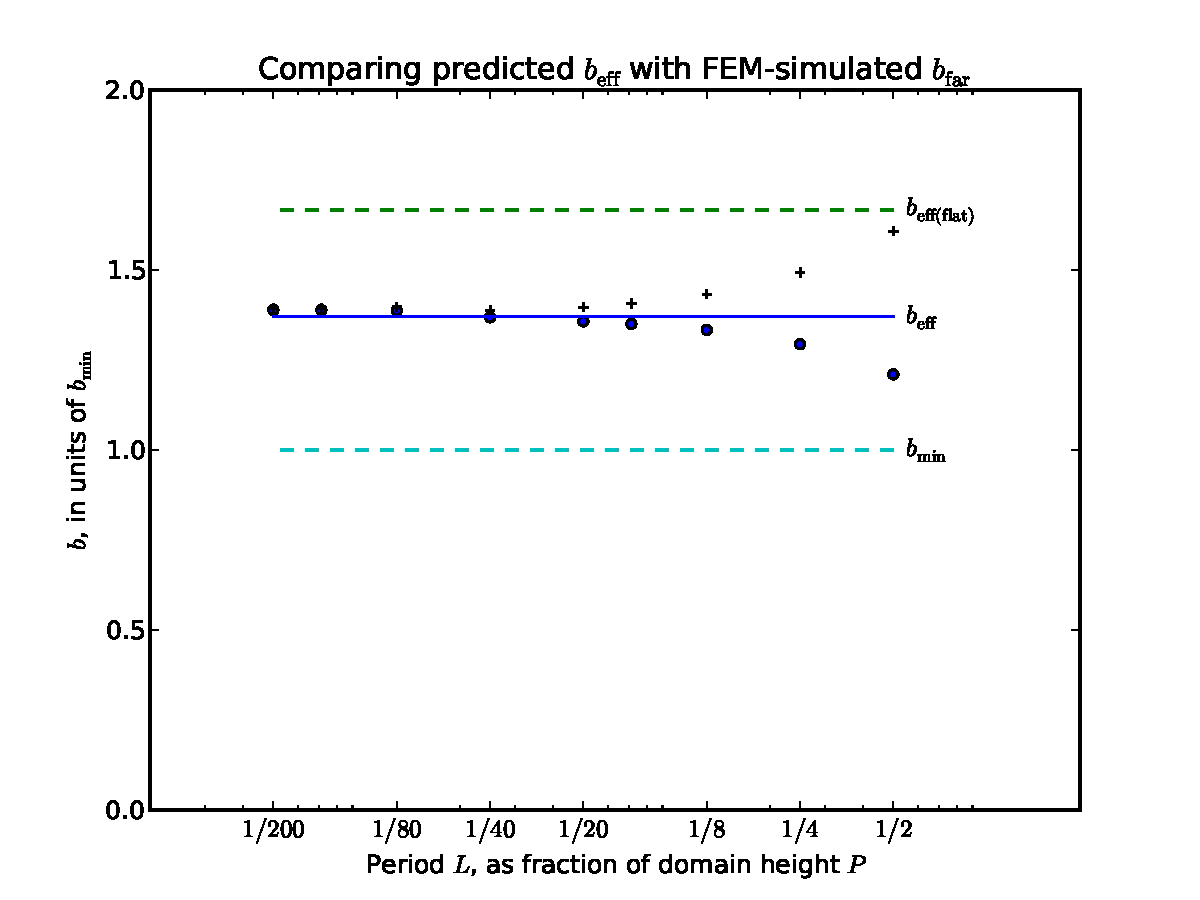
\includegraphics[scale=0.595]{Lund_Thesis_FEM_plot_sine_corr}
% Absurd scale factor is to suppress the error message!
\caption{Comparison of numerical $\bfar$ values with $\beff$ predictions for \textbf{sinusoidal} surfaces for different periods, with $b\sim P$. The dots are values of $\bfar$ calculated w.r.t. the $z=0$ line, and the crosses are $\bfar$ values calculated w.r.t. the top of the sinusoid. The solid line is the $\beffha$ prediction.  The upper dashed line is the $\beffhf$ predicted if the surface were assumed to be flat.}\label{FEMplotsinecorr}
\end{figure}

Figure (\ref{FEMplotsinecorr}) shows that the slip lengths defined with respect to the tops of the surface peaks differ from the predicted $\beff$ by about the same amount as the $z=0$ based slip lengths -- but in the other direction.
In other words, for a given period $L$, the predicted $\beff$ value lies between the two numerical $\bfar$ values calculated with respect to the two different reference points.  The difference between the two types of $\bfar$ values increases as $L$ increases, because the roughness amplitude increases in concert. 
The accuracy of $\beff$ depends on how the measured $\bfar$ values are calculated, and
the `correct' way to calculate $\bfar$ depends on the circumstance.  If effective slip lengths are measured with respect to the tops of the roughness, then our $\beff$ predictions will underestimate measured effective slip lengths. 
%; without being quantitative, Figure (\ref{FEMplotsine3}) suggests that neither of the two types of $\bfar$ considered give rise to significantly better accuracy than the other. 

%\clearpage
A final note about numerical issues:  A close look look at the data plotted in Figure (\ref{FEMplotsinepcnt}) reveals that the numerics and the prediction agree better and better as $L$ gets smaller and smaller --- up to a point.  Then the prediction \emph{underestimates} the numerical values.  We believe this to be a computational artefact, due to an insufficient number of lattice points  on a very rapidly oscillating boundary:  When we noticed that the $\bfar$ values overshot the prediction, we ran the same simulations with double the number of lattice points.  The overshoot reduced, so we further increased the number of lattice points, which gave even better results.  At some point we hit the limit of our computational power, but it is reasonable to think that given sufficient computational power, the discrepancy would disappear.
  
%As the FEM simulations were tuned using finer and finer mesh granularity, the $\bfar$ values overshot $\beff$ by less and less, suggesting that the overshoot is due to an insufficient number of lattice points on a very rapidly oscillating boundary.

%As the simulations were tuned, using finer and finer mesh granularity, in the regime $L \ll P$, the $\bfar$ values got closer and closer to predicted $\beff$ (overshooting by less and less).  Extrapolating to the limit of infinite computing power, we suggest that the numerics would \emph{never} overshoot $\beff$, and the overshoot seen here is due to an insufficient number of lattice points on a very small and rapidly oscillating sine wave boundary.








\clearpage
\section{Finite Difference Numerics}

As an exercise, the same slip problem was also solved numerically using the finite difference method.  The main benefit of this exercise (apart from educational) was that the software employed allowed the easy visualisation of 3-dimensional flow fields.  We employed Python using the Numpy library, which is a front end to various very fast C and Fortran libraries, and the Mayavi library for visualisation.  A curved boundary is difficult to implement in this approach, so the case of the flat slip boundary was studied.

Three-dimensional velocity profiles were generated.  The $x$-velocity $u$ for flow over a mixed-slip surface is shown in Figure (\ref{flow}).

\begin{figure}[ht]
\centering
\begin{tikzpicture}
\node [above right] { 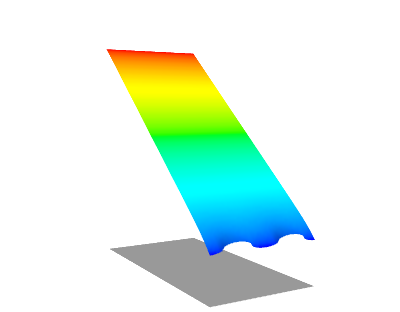
\includegraphics[scale=0.595]{Lund_Thesis_Flow} };

\coordinate (origin) at (4.53,0.22);
\draw[->] (origin) -- node[below]{$x$} ++(11:3cm);
\draw[->] (origin) -- node[below]{$z$} ++(150:2.5cm) -- node[left]{$u$} ++(0,5);
\draw (origin) ++(150:2.5cm) ++(0,4.17) -- ++(-0.15,0) node[left] {$u_P$};

\node at (6.8,1.65)[right]{$u$ with mixed-slip boundary};
\end{tikzpicture}
\caption{The coloured surface is $u$, the $x$-velocity component of a velocity field of a finite difference simulation of flow over a flat mixed-slip surface.}\label{flow}
\end{figure}


The $x$-velocity is high and uniform at the top boundary condition (large $z$), and varies periodically over the slip boundary.

\clearpage
To provide some perspective, flow profiles over \emph{pure} high-slip and low-slip surfaces were generated.  These are plotted together, along with the mixed-slip flow profile, in Figure (\ref{flowhilo}).

\begin{figure}[ht]
\centering
\begin{tikzpicture}
\node [above right] { 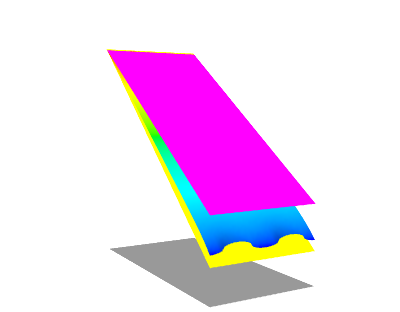
\includegraphics[scale=0.595]{Lund_Thesis_Flow_HiLo} };

\coordinate (origin) at (4.53,0.22);
\draw[->] (origin) -- node[below]{$x$} ++(11:3cm);
\draw[->] (origin) -- node[below]{$z$} ++(150:2.5cm) -- node[left]{$u$} ++(0,5);
\draw (origin) ++(150:2.5cm) ++(0,4.15) -- ++(-0.15,0) node[left] {$u_P$};

\node at (6.6,2.7)[right]{$u$ with high-slip boundary};
\node at (6.6,1.8)[right]{$u$ with mixed-slip boundary};
\node at (6.6,1.25)[right]{$u$ with low-slip boundary};

\end{tikzpicture}
\caption{The same mixed-slip flow field as in Figure (\ref{flow}), plus the flow solutions for flow over the purely high-slip surface (pink), and the purely low-slip surface (yellow).}\label{flowhilo}
\end{figure}

There is an interesting feature in the mixed-slip flow field: while the velocity at the slip boundary varies periodically, the variation is not very large.  The slip velocity does \emph{not} swing between the extremes of velocities over the pure high-slip and low-slip surfaces.  Instead, the slip velocity has only a moderate periodic variation about a central value.

What is that central value?  Of course, we expect it to be the slip velocity that would occur if the surface had a single slip length equal to our predicted $\beff$.
We explore this by generating a last flow profile with a pure $\beff$ slip length surface.  We plot this (in black) together with the mixed-slip flow profile in Figure (\ref{floweff}).

\clearpage
\begin{figure}[ht]
\centering
\begin{tikzpicture}
\node [above right] { 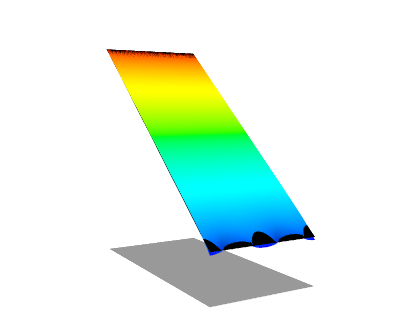
\includegraphics[scale=0.595]{Lund_Thesis_Flow_Eff} };

\coordinate (origin) at (4.53,0.22);
\draw[->] (origin) -- node[below]{$x$} ++(11:3cm);
\draw[->] (origin) -- node[below]{$z$} ++(150:2.5cm) -- node[left]{$u$} ++(0,5);
\draw (origin) ++(150:2.5cm) ++(0,4.17) -- ++(-0.15,0) node[left] {$u_P$};

\node at (6.7,1.9)[right]{$u$ with $\beff$ slip boundary (black)};
\node at (6.6,1.45)[right]{$u$ with mixed-slip boundary};
\end{tikzpicture}
\caption{The same mixed-slip flow field as in Figure (\ref{flow}), plus the flow field corresponding to a homogeneous boundary of slip length $\beff$ (black).}\label{floweff}
\end{figure}

Figure (\ref{floweff}) shows excellent agreement between the effective flow profile and the mixed-slip profile.  For most of the domain, they are almost indistinguishable.  Only very close to the slip boundary does the mixed-slip profile exhibit a periodic variation about the effective slip profile.

\vspace{1em}

The plot of Figure (\ref{floweff}) also throws light on another issue: how thick is the boundary layer?  The boundary layer can be  arbitrarily defined to end where the flow becomes (arbitrarily close to) uniform.  Without being quantitative, we can see that a reasonable choice for boundary layer thickness $d$ could be less than the period $L$.
%  This would explain why the FEM simulations showed that $\beff$ works unexpectedly well even when it is not strictly true that $L \ll \bmin$.  The explanation is that even when $L \sim \bmin$, it may still be true that $d < \bmin$.  

%Finally, recall that the condition $L \ll \bmin$ is not a `requirement' as such.  In the mathematical model, $L$ and $\bmin$ are the appropriate nonarbitrary length scales, and the expression for $\beff$ becomes more and more exact as $L \to 0$.  To summarise the concept `$L$ is closer to zero than $\bmin$ is close to zero', one simply states that $L \ll \bmin$.


\clearpage
\section{Conclusion}

Numerical simulations reveal that if the period of surface patterning $L$ is much less than the domain height $P$ and typical slip lengths, then the effective slip length as defined in the far field of the system is very well approximated by:
\begin{equation}
\beff = \left<  \frac{\sqrt{1 + |\nabla h  |^2}}{b} \right> ^{-1}
\label{eq:harm}
\end{equation}
The $\beff$ expression incorporates a correction for the increased area of solid-liquid contact in rough surfaces.  Numerical testing shows this correction to be accurate, so therefore our $\beff$ expression of Equation (\ref{eq:harm}) is valid for both flat and rough surfaces.

Numerical simulations further reveal that if $L \ll P$ and slip lengths are of the same order as the period, $L \sim b$, then Equation (\ref{eq:harm}) is a surprisingly good approximation for effective slip lengths.

If slip lengths are much smaller than any other length scale, then the effective slip length is best approximated by a simple area-weighted mean.  Numerical testing with a flat surface showed that if $\bmax \leq \frac{1}{40} \ll P$, then the effective slip length is well approximated by:
\begin{equation}
\beff = \langle b \rangle
\end{equation}




\iftoggle{compilealone}
    {
    \bibliography{Lund_Thesis.bib}
    \bibliographystyle{plain}
    }

\end{document}




\clearpage
\subsection{Rough Surface (Old)}

Using FreeFem++, we modelled a two-dimensional fluid.  The fluid was driven by a fixed shear rate at the top boundary.  The slip boundary at the bottom was a sine wave profile, with an intrinsic slip length that varied in a binary fashion with the same period: The slip length on the peak of the sine wave was a low value, and the slip length on the trough of the sine wave was a high value.  This models shear-driven flow transverse to a grating or corrugation, with an air pocket in the grooves. 
A schematic is shown in Figure (\ref{FEMmodel}).


\begin{figure}[ht]
\centering
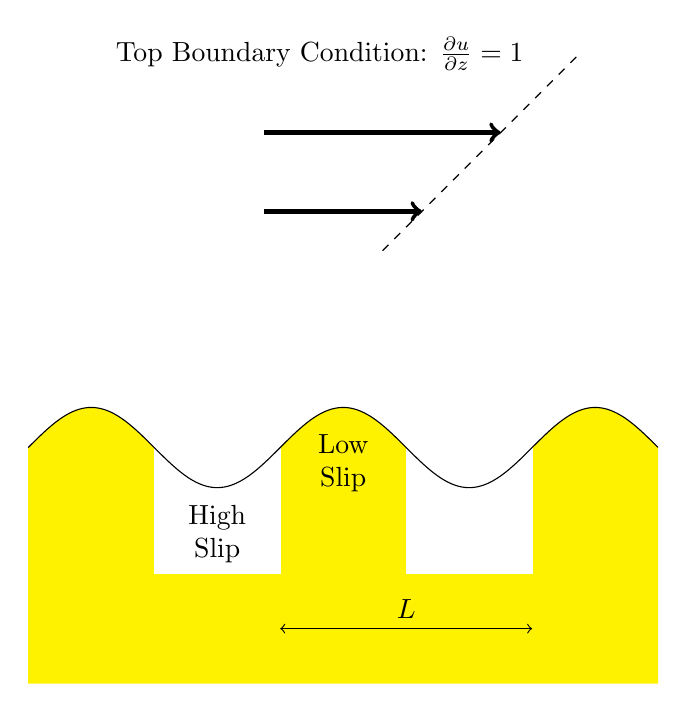
\begin{tikzpicture}
\node at (3.7,5) {Top Boundary Condition: $\frac{\partial u}{\partial z} = 1 $};

\draw[->, ultra thick] (3,4) -- ++(3,0);
\draw[->, ultra thick] (3,3) -- ++(2,0);
\draw[dashed] (3,2.5) ++(1.5,0) -- ++(2.5,2.5);

% \L = 3.2; length of period
\fill [color=yellow,domain=0:8,samples=200] plot (\x,{ (3.2 /6.2823) * sin( 6.2832 *\x / 3.2 r)} ) -- ++(0,-3) -| (0,0);

\draw[color=white,fill=white] (1.6,0) rectangle ++(1.6,-1.6);
\draw[color=white,fill=white] (4.8,0) rectangle ++(1.6,-1.6);

\draw [domain=0:8,samples=200] plot (\x,{ (3.2 /6.2823) * sin( 6.2832 *\x / 3.2 r)} );

\draw[<->] (3.2,-2.3) -- node[above] {$L$} ++(3.2,0);

\renewcommand{\baselinestretch}{1.00}
\node at (2.4,-1.1) [align=center] {High \\ Slip};
\node at (4,-0.2) [align=center] {Low\\ Slip};


\end{tikzpicture}
\caption{Schematic of the model used in the finite element analysis.}\label{FEMmodel}
\end{figure}

\clearpage
Specifics:  The minimum slip length was $\bmin = 1$, the maximum slip length was $\bmax = 5$, the   height of domain was $P = 20$, and the fixed shear rate at $P$ was 1 s$^{-1}$.  The sinusoidal surface was centered at $z=0$, with $\bmin$ on the peaks and $\bmax$ in the troughs.   With $\bmax$ at 25\% of domain height $P$, this regime is \emph{not} near the limit of vanishing slip length, so we expect the homogenized area-weighted harmonic mean formula to apply.  The formula predicts $\beff = 1.36$.

The FEM analysis was done for a series of sinusoidal slip surfaces, each with a different period $L$, but with the same values of $\bmin$ and $\bmax$.  For each $L$, an effective slip length $\bfar$ was calculated from the far-field velocity field solution. These are plotted as the dots in Figure (\ref{FEMplot}).  
The predicted $\beff$ appears as a solid line.  
Period $L$ is expressed as a fraction of $P$.

%The FEM solution for each surface is a velocity field; from the far-field part of this solution an effective slip length $\bfar$ was calculated. 
% The fixed slip lengths and the sine wave profile were plugged into our formula, generating $\beff$.  The results are plotted in Figure (\ref{FEMplot}).  The solid line is the predicted $\beff$ (which does not depend on $L$), and the dots are the simulated $\bfar$ values at various values of $L$.


\begin{figure}[ht]
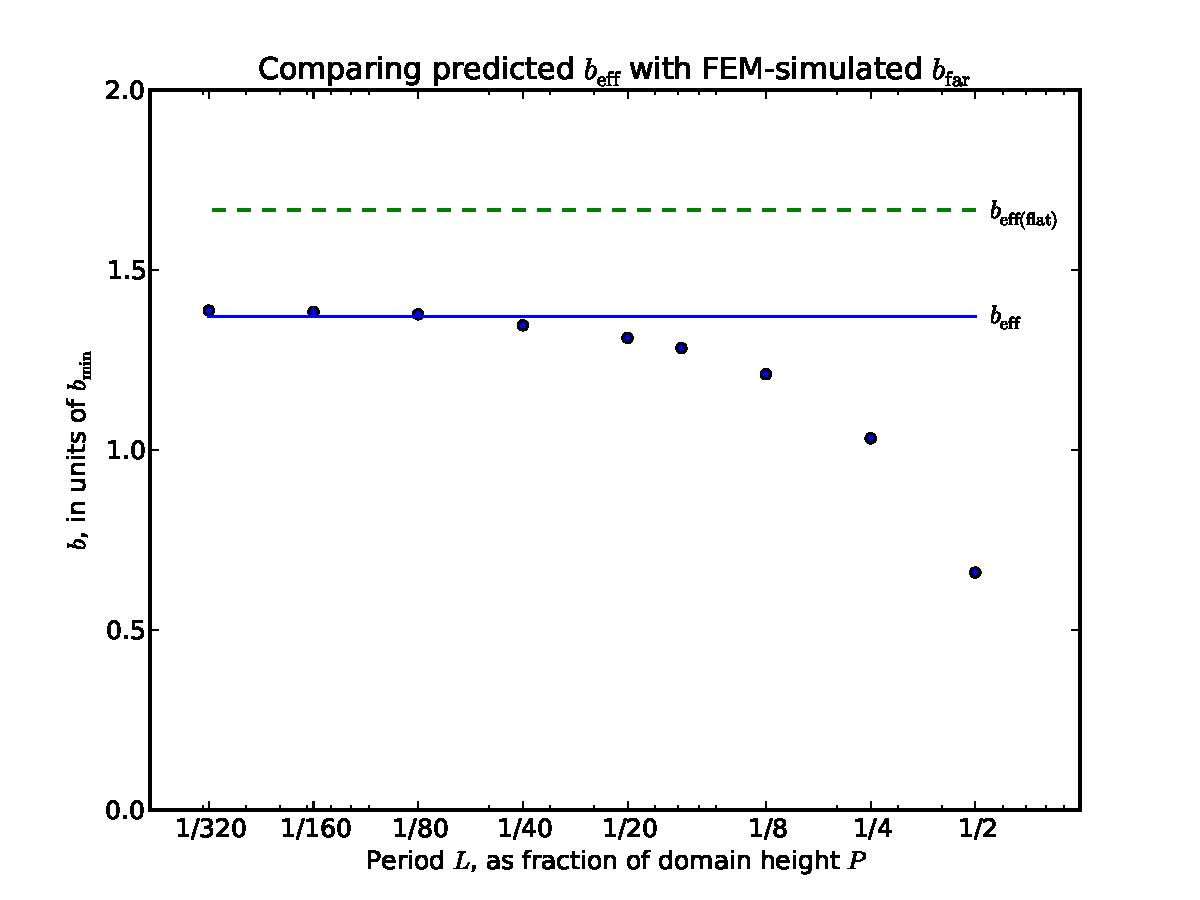
\includegraphics[scale=0.595]{Lund_Thesis_FEM_plot_LonP}
% Absurd scale factor is to suppress the error message!
\caption{Dots are values of $\bfar$ -- the effective slip length values calculated from the far-field velocity solutions of FEM simulations.  Solid line is the predicted $\beff$.  Dotted line is the $\beff$ predicted if the surface were assumed to be flat. }\label{FEMplot}
\end{figure}

As noted, a system is `near the limit' if $L \ll P$, in which case the predicted $\beff$ should approximate measured $\bfar$ very well.  Figure (\ref{FEMplot}) shows this to be true.

%As noted, a system is `near to the limit' if $L \ll \bmin$, in which case the predicted $\beff$ should approximate measured $\bfar$ very well.  This is true.  At $L = 0.1 \bmin$, the plot shows the numerically-calculated $\bfar$ (dots) to be within a few percent of predicted $\beff$ (solid line).

For interest,
the dashed green line is the effective slip length calculated if the surface were naively assumed to be flat.  Comparison with the numerical values shows the importance of the correction from using true contact area: the naive flat calculation overshoots numerical slip lengths by about 20\%.



%But the pleasant surprise is that our full roughness-corrected $\beff$ prediction appears to be good even where $L \sim \bmin$.
%For ease of comparing relative magnitudes, in Figure (\ref{FEMplotpcnt}) we plot the data with $\bfar$ expressed as a percentage difference from $\beff$.


To better quantify the success of our $\beff$ prediction, we plot the same data with $\bfar$ expressed as a percentage difference from $\beff$.  This is shown in Figure (\ref{FEMplotpcnt}).

\begin{figure}[ht]
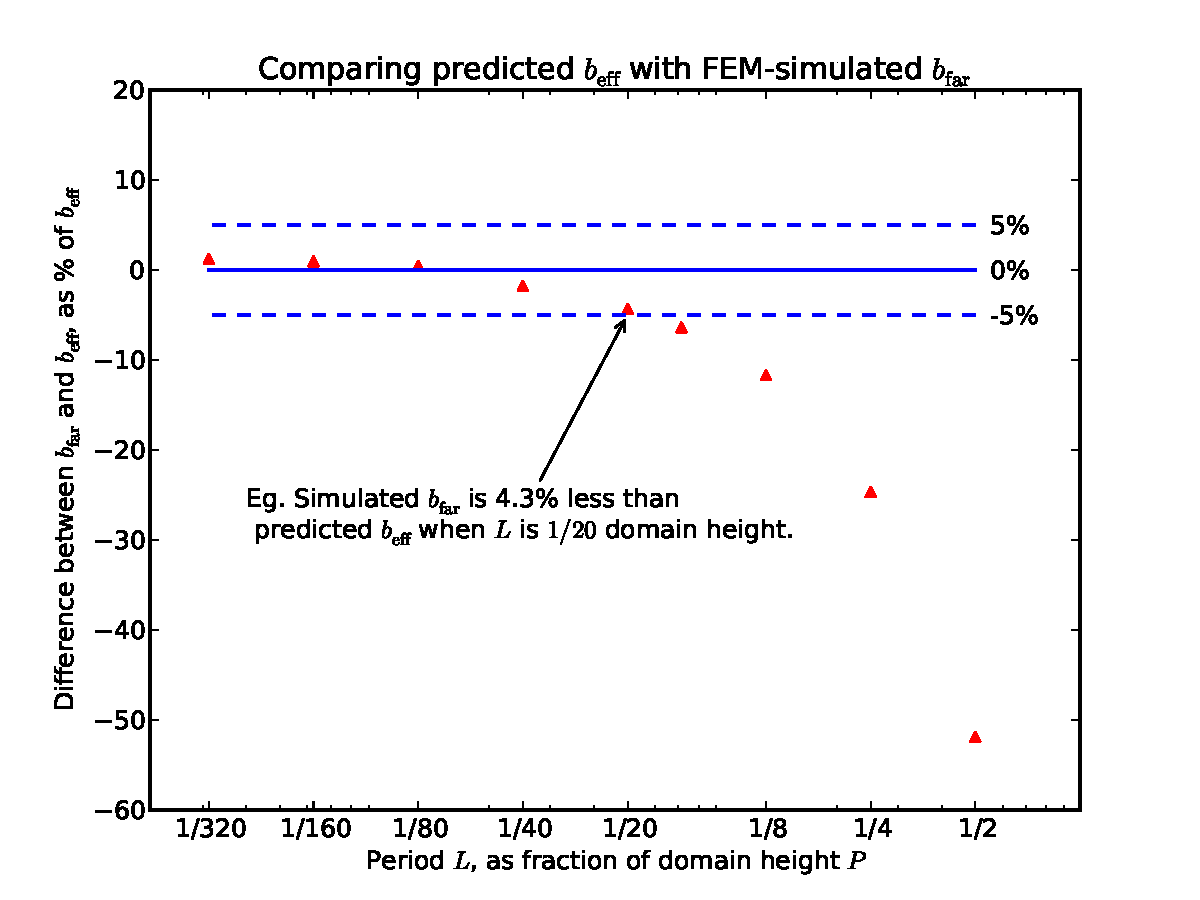
\includegraphics[scale=0.595]{Lund_Thesis_FEM_plot_pcnt_LonP}
% Absurd scale factor is to suppress the error message!
\caption{Triangles are values of $\bfar$ -- effective slip lengths from FEM simulations.  Solid line is predicted $\beff$.  Dashed lines are 5\% above and below $\beff$.}\label{FEMplotpcnt}
\end{figure}

We see that if $L$ is 5\% of $P$, then the numerical results differ from our prediction by less than 5\%.
In fact the data suggest a rough rule of thumb: if $L$ is $x$\% of $P$, measured $\bfar$ will be $x$\% less than predicted $\beff$.



%So, while \emph{a priori} we can only expect our prediction to be trustworthy if $L \ll \bmin$, in practice --- or at least in this numerical simulation --- our prediction is very good for much larger values of roughness period, where $L \leq \bmin$.

%\clearpage
The slip lengths in these FEM simulations were calculated with respect to the $z=0$ line, about which the sinusoids oscillate.  In Chapter \ref{C:mixedslip} we noted the ambiguity in the definition of slip length -- does the surface begin at the $z=0$ line or at the tops of the sine wave peaks?  To investigate this issue, we recalculated the measured slip lengths with respect to the \textbf{tops of the peaks}.  These are plotted as the crosses in Figure (\ref{FEMplotcorrected}) (along with the `uncorrected' slip lengths).

\begin{figure}[ht]
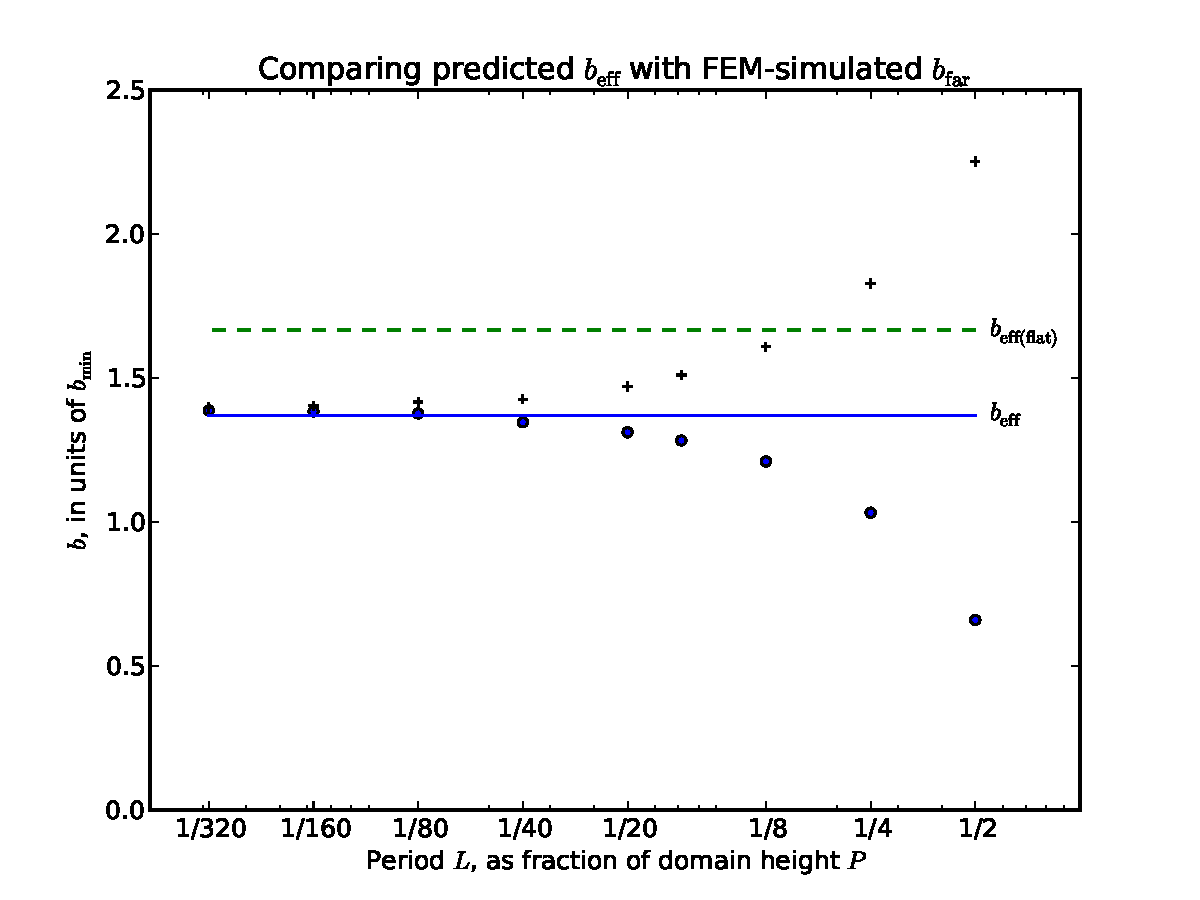
\includegraphics[scale=0.595]{Lund_Thesis_FEM_plot_LonP_corrected}
% Absurd scale factor is to suppress the error message!
\caption{Dots are values of $\bfar$, as in Figure (\ref{FEMplot}).  Crosses are $\bfar$ calculated w.r.t the tops of the surface peaks.  Solid line is the predicted $\beff$.  Dotted line is the $\beff$ predicted if the surface were assumed to be flat. }\label{FEMplotcorrected}
\end{figure}

Figure (\ref{FEMplotcorrected}) shows that the slip lengths defined with respect to the tops of the surface peaks differ from the predicted $\beff$ by about the same amount as the $z=0$ based slip lengths -- but in the other direction.  The good news is that our predicted $\beff$ is pretty much in the middle of the defensible range of measured slip lengths.


Note that while the homogenized $\beff$ is expected to work when $L \ll P$, the perturbation method \emph{assumed} $L \ll P$, and the result was considered valid when $b \sim P$.  The example here, with $\bmin$ = 10\% of $P$, and $\bmax$ = 25\% of $P$, is on the borderline of this requirement.  But the result still works excellently.  This suggests that the requirement of the perturbative result is not fundamental, and affirms that homogenization is a stronger technique. 

A final note about numerical issues:  A close look look at the data plotted in Figures (\ref{FEMplot}) and (\ref{FEMplotpcnt}) reveals that the numerics and the prediction agree better and better as $L$ gets smaller and smaller --- up to a point.  Then the prediction \emph{underestimates} the numerical values.  We believe this to be a computational artefact.  As the simulations were tuned, using finer and finer mesh granularity, in the regime $L \ll P$, the $\bfar$ values got closer and closer to predicted $\beff$ (overshooting by less and less).  Extrapolating to the limit of infinite computing power, we suggest that the numerics would \emph{never} overshoot $\beff$, and the overshoot seen here is due to an insufficient number of lattice points on a very small and rapidly oscillating sine wave boundary.
